\section{Ejercicio 7}
	Computaciones para el programa
	\begin{verbatim}
	J(2,3,9)
	J(1,3,9)
	S(3)
	S(4)
	J(2,4,7)
	J(1,1,2)
	Z(4)
	J(1,1,2)
	T(4,1)
	\end{verbatim}
	\subsection{Computación para la entrada $R1=0$, $R2=0$}
	\begin{equation*}\begin{gathered}
	(1, <R1=0, R2=0, R3=0, R4=0>) \sim (9, <R1=0, R2=0, R3=0, R4=0>) \sim\\
	(10, <R1=0, R2=0, R3=0, R4=0>)
	\end{gathered}\end{equation*}
	\begin{figure}[H]
  		\centering
  		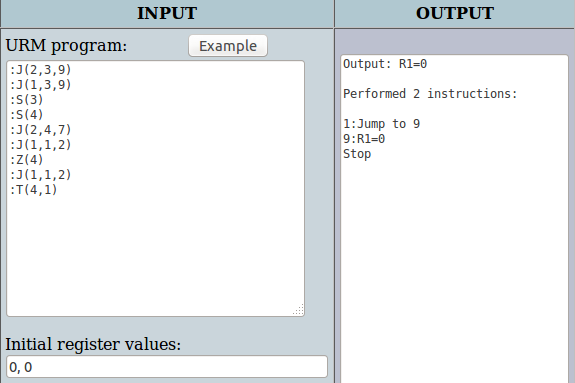
\includegraphics[scale=0.5]{images/700.png}
  	\end{figure}
	\subsection{Computación para la entrada $R1=0$, $R2=1$}
	\begin{equation*}\begin{gathered}
	(1, <R1=0, R2=1, R3=0, R4=0>) \sim (2, <R1=0, R2=1, R3=0, R4=0>) \sim\\
	(9, <R1=0, R2=1, R3=0, R4=0>) \sim (10, <R1=0, R2=1, R3=0, R4=0>)
	\end{gathered}\end{equation*}
	\begin{figure}[H]
  		\centering
  		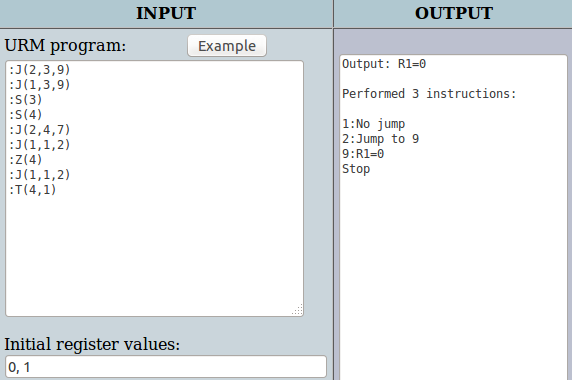
\includegraphics[scale=0.5]{images/701.png}
  	\end{figure}
	\subsection{Computación para la entrada $R1=1$, $R2=0$}
	\begin{equation*}\begin{gathered}
	(1, <R1=1, R2=0, R3=0, R4=0>) \sim (9, <R1=1, R2=0, R3=0, R4=0>) \sim\\
	(10, <R1=0, R2=0, R3=0, R4=0>)
	\end{gathered}\end{equation*}
	\begin{figure}[H]
  		\centering
  		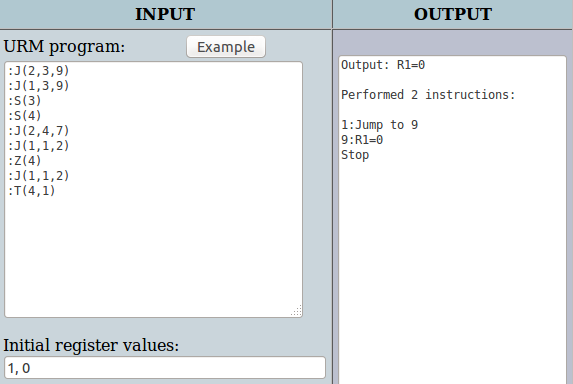
\includegraphics[scale=0.5]{images/710.png}
  	\end{figure}
	\subsection{Computación para la entrada $R1=1$, $R2=1$}
	\begin{equation*}\begin{gathered}
	(1, <R1=1, R2=1, R3=0, R4=0>) \sim (2, <R1=1, R2=1, R3=0, R4=0>) \sim\\
	(3, <R1=1, R2=1, R3=0, R4=0>) \sim (4, <R1=1, R2=1, R3=1, R4=0>) \sim\\
	(5, <R1=1, R2=1, R3=1, R4=1>) \sim (7, <R1=1, R2=1, R3=1, R4=1>) \sim\\
	(8, <R1=1, R2=1, R3=1, R4=0>) \sim (2, <R1=1, R2=1, R3=1, R4=0>) \sim\\
	(9, <R1=1, R2=1, R3=1, R4=0>) \sim (10, <R1=0, R2=1, R3=1, R4=0>)
	\end{gathered}\end{equation*}
	\begin{figure}[H]
  		\centering
  		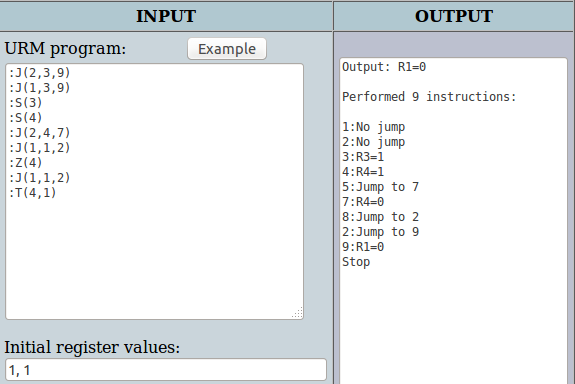
\includegraphics[scale=0.5]{images/711.png}
  	\end{figure}
	\subsection{Función calculada}
	El programa calcula la función
	\begin{equation*}
		f(x_1, x_2)= \left\{ 
  		\begin{array}{rl}
  				x_1 \bmod x_2 & \text{si } x_2>0 \\
  				0 & \text{en otro caso} 
  		\end{array} \right.
	\end{equation*}
